\section{B\'usqueda y Pateo}\label{chapter:busqueda}

Para poder buscar y patear la pelota, además de tener la capacidad para detectarla (como se explicó en la secci\'on anterior anterior), debe ser capaz de moverse en su entorno, poder patear, levantarse, tener una representación del mundo que lo ayude a orientarse y tener una estrategia para elegir el conjunto de movimientos que lo lleven a acercarse a la pelota. 

En esta sección se explica el desarrollo de las actividades que han sido necesarias para ejecutar la búsqueda y pateo de la pelota.
%, con excepción de la estrategia para la toma de acciones, que se explicará en la sección \ref{aprendizaje}.

Primero, en la sección \ref{subsection:Herrbusqueda} se da una breve descripción de las herramientas de software que apoyaron las tareas de búsqueda y pateo. En la sección \ref{esqueleto} se explica cuál fue el conjunto de movimientos creados para el esqueleto del robot.

El sensor principal de Junny, es el observador de su ambiente, la c\'amara. \'Esta tiene dos grados de libertad para su movimiento, lo que causa que tenga un gran número de posibles posiciones. Para simplificar, se ha límitado la cantidad de posiciones. En la secci\'on \ref{movCamara} se explica las posiciones que puede adoptar la cámara. Luego en la secci\'on \ref{mundo} se explica la manera en la que Junny organiza la representaci\'on visual que capta del mundo.

Debido a que el movimiento del robot se controla desde la tarjeta Arbotix y la detecci\'on de la pelota se hace desde la Raspberry Pi, se debi\'o establecer la comunicaci\'on entre ambas tarjetas. Este proceso se explica en la secci\'on \ref{comunicacion}.

Una vez con la representaci\'on del mundo, los movimientos programados y la comunicaci\'on de las tarjetas, solo faltaría decidir que acci\'on tomar en cada situación. La estrategia, basada en el paradigma h\'ibrido, se explica en la secci\'on \ref{eleccionAccionesFijas}.        

%Como se mencion\'o anteriormente el robot debe buscar y patear una pelota de tamaño de una pelota de tennis y ya se ha descrito las caracter\'isticas f\'isicas y de software que utiliza el robot, esta secci\'n se enfoca en el comportamiento que describe a este robot.
%Para ello primero se especifica la serie de movimientos implementados y el comportamiento que lo representa.
 
\subsection{Herramientas software para la b\'usqueda de la pelota } \label{subsection:Herrbusqueda}

Para cumplir con el desarrollo de la programación de la búsqueda y pateo de la pelota, se han utilizado algunas herramientas que han facilitado el proceso. A continuación se describen las más destacadas dentro del proyecto. 

\begin{itemize}
\item Pypose: Software especializado en el control de los servomotores Dynamixel Ax-12. Una de las más importantes características es que, luego de haber fijado a mano las posiciones de los motores, permite la lectura simultánea de esas posiciones para captar la pose del robot. Con esta herramienta es posible formar una secuencia de poses que generen un movimiento, por ejemplo, caminar \cite{pypose}. 

\item IDE Arduino: Es un entorno de desarrollo para escribir y cargar código en la tarjeta Arduino. Otras tarjetas con microcontroladores AVR también son compatibles, como la Arbotix. El lenguaje de programación del IDE de Arduino es una implementación de Wiring el cual está basado en Processing \cite{arduino}.  


\item ROS: ROS (Robot Operating System) es un Framework flexible para la escritura de software enfocado en robots. Es una colección de herramientas, bibliotecas y convenciones que tienen por objeto simplificar la tarea de crear un comportamiento complejo y robusto a través de una amplia variedad de plataformas robóticas. ROS se encuentra bajo licencia de código abierto, la licencia BSD \cite{ros}.

\item HServo: Es una librería de código libre distribuida bajo la Licencia Pública General Reducida de GNU. Esta librería se encuentra desarrollada especificamente para la tarjeta Arbotix, ya que con la nueva librería de Arduino Servo se pueden experimentar fallas en el control de los servos. La interfaz es la misma, la diferencia es que solo puede ser usada para servos conectados en los pines 12 y 13 de la tarjeta Arbotix \cite{HServo}.    

\end{itemize}

%\subsection{Comportamiento}

%Debupa es un robot humanoide implemetado de forma autonoma e inteligente que sigue un comportamiento bajo el paradigma h\'ibrido (secci\'on 2 ). El sensor principal (c\'amara ) es el observador del mundo, que posee una serie de movimentos determinados (secci\'on REF) con los cuales escanea el mundo y combinados con la serie de movimiemtos del esqueleto es capaz de encontrar la pelota. Al determinar la posici\'on de la pelota Debupa logr\'o aprender (secci\'on APRENDIZAJE) la mejor acci\'on a relizar para estar mas cerca de ella y al llegar poder patearla.

\subsection{Movimiento del esqueleto}\label{esqueleto}

El robot debe tener la capacidad de ejecutar una variedad de movimientos para poder cumplir la meta de patear la pelota. Por ello se ha programado un conjunto de poses y transiciones o acciones de movimiento que se explican a continuación.

Con fines explicativos, en este proyecto, la palabra ``pose" se referire a la posición específica de los 16 motores que constituyen el esqueleto del robot. Un conjunto de poses ejecutadas en secuencia se denominará ``acción de movimiento".

Las acciones de movimiento establecidas son:

\begin{itemize}
% \item {Caminar 2.5 cm hacia adelante }
 \item {Caminar dos pasos hacia adelante (4.8 cm ) }
% \item {Caminar 9.9 cm hacia adelante }
 \item {Girar a la izquierda (3 cm)}
% \item {Girar 6 cm a la izquierda} 
 \item {Girar a la derecha (3 cm)}
% \item {Girar 6 cm a la derecha}	 
 \item {Levantarse desde la posición boca abajo}
 \item {Levantarse desde la posición boca arriba}
 \item {Patear con la pierna derecha }
 \item {Patear con la pierna izquierda}
 
\end{itemize}

Estas poses han sido fijadas a través de la tarjeta controladora Arbotix y el software Pypose. De esta manera se ha fijado y guardado un conjunto de poses para cada acción de movimiento. Estas acciones de movimientos han sido exportadas para ser utilizadas en el programa, en lenguaje Wiring, a ser ejecutado en Arbotix. La programación en Arbotix se ha realizado bajo el ambiente del IDE de Arduino. 


\subsection{Movimiento de la cámara}\label{movCamara}
La cámara ha sido instalada sobre dos micro servomotores analógicos, otorgándole dos grados de libertad. El servomotor ubicado en la parte inferior se encarga del movimiento horizontal y el superior, del movimiento vertical.

El hecho de  que la cámara tenga dos grados de libertad para moverse es una gran ventaja, ya que se puede obtener un mayor rango de visión. Junny puede mirar hacia la derecha o izquierda sin tener que mover sus piernas, también puede mirar hacia abajo para verificar que la pelota esté en sus pies, para patear, o hacia arriba para ubicar la pelota a mayor distancia.

El número de posibles posiciones para la cámara es muy amplio y para simplificar se ha reducido a 6 posiciones fijas, cuya distribución obedece al objetivo de que la cámara obtenga una amplia visión, sin dejar espacios no visibles. Esta simplificación ayuda en la tarea de la representación del mundo que se explica en la sección \ref{mundo}. En la figura~\ref{posicionesCam} se puede observar la cámara del robot en las diferentes posiciones que se han fijado para ella.  

\begin{figure}[hbtp]
\centering
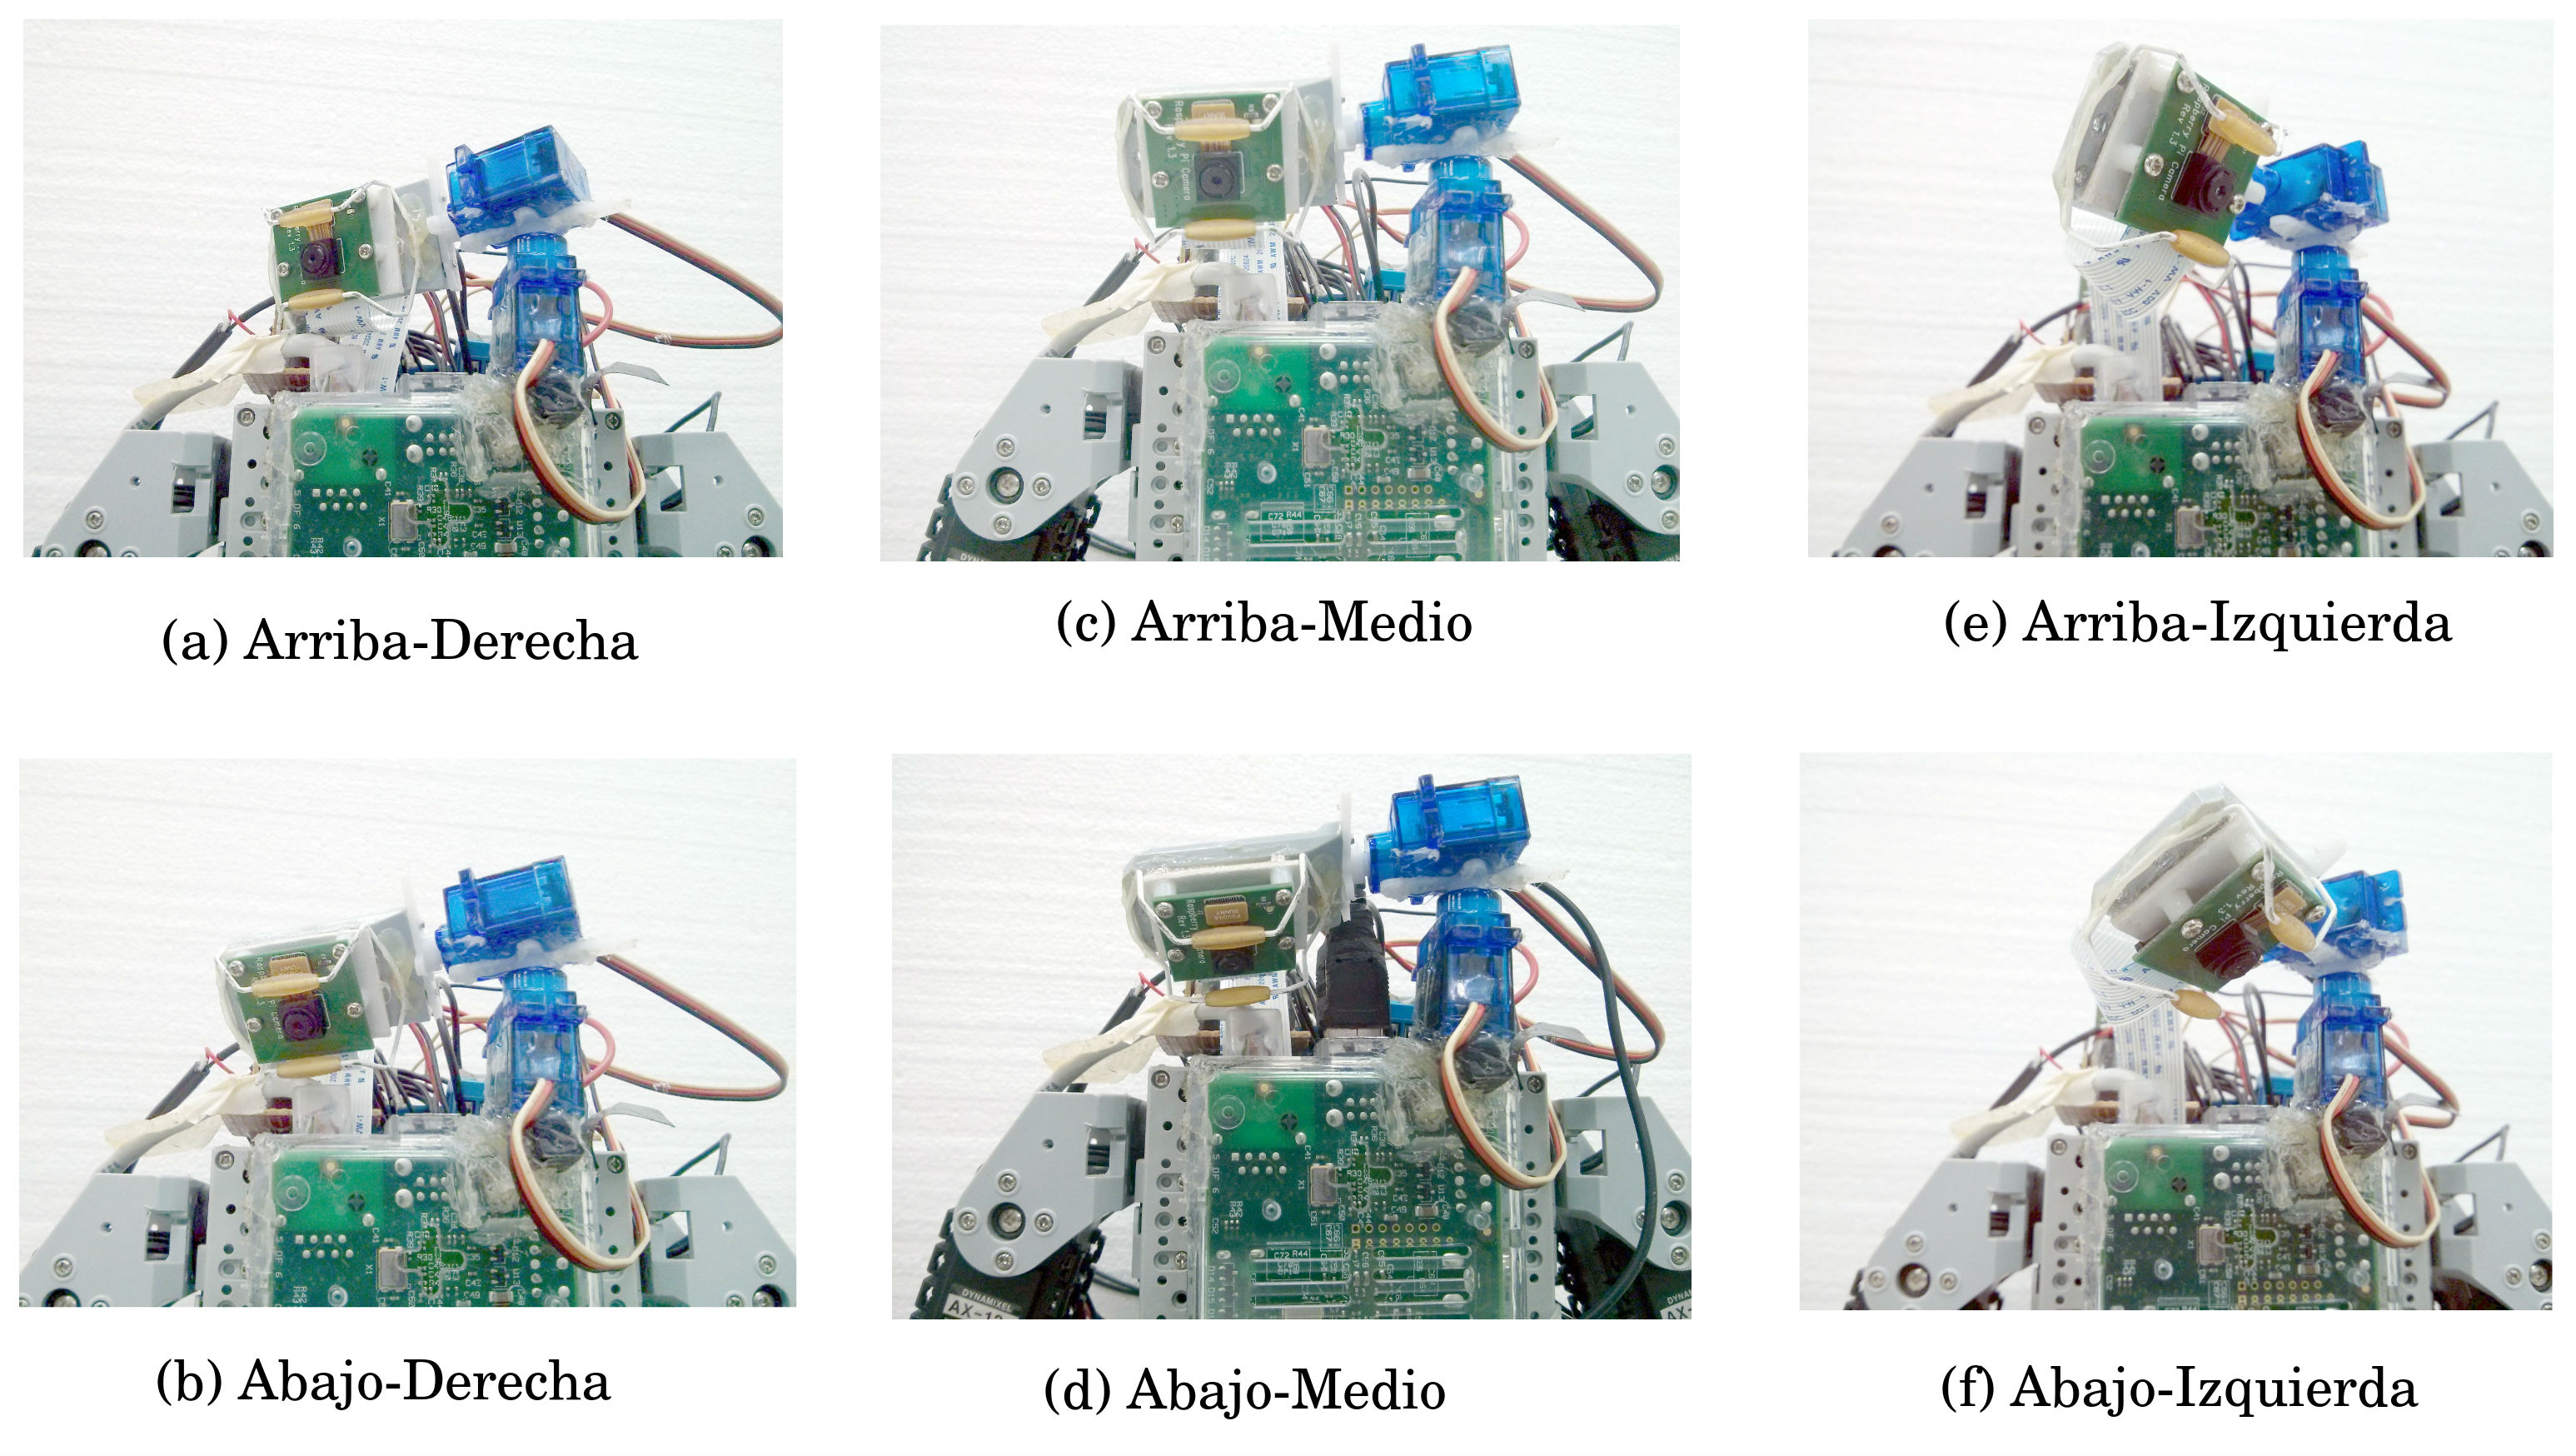
\includegraphics[scale=0.14]{imagenes/posicionesCamara.jpg}
\caption{Posiciones de la cámara }
\label{posicionesCam}
\end{figure}

Los micro servomotores azules que aparecen en la imagen \ref{posicionesCam} se controlan desde la Arbotix usando la librería HServo. Esta librería s\'olo puede ser usada para los motores conectados en los puertos Hobby A y B (pines 12 y 13) (ver la figura ~\ref{fig:arbotixConectados}). Tener los motores conectados a estos puertos brinda la ventaja de un control más preciso, evitando que los motores generen vibración, ya que los pulsos son generados por temporizadores de hardware. 

\subsection{Representaci\'on del mundo}\label{mundo}

La representación del mundo de Junny se basa en función de la posición de la pelota con respecto al él. 

La cámara tiene 6 (2x3) posibles posiciones, como se muestra en la figura ~\ref{posicionesCam} y desde cada posición de la cámara se obtiene una imagen. La detección de la pelota en alguna de esas imagenes brinda una orientación sobre la ubicación de la pelota. Si se detecta la pelota, por ejemplo, cuando la cámara se encuentra en alguna de las posiciones de la derecha, es un indicativo de que la la pelota se encuentra a la derecha y que si el robot gira se podría posicionar frente a ella. 

Se ha decidido discretizar las posibles posiciones de la pelota por regiones. Estas regiones se muestran enumeradas en la fugura ~\ref{divisionCam}. Cada cuadro blanco demarcado por líneas negras representa la imagen captada en una posición fija de la cámara. 

Las imagenes de la cámara en la posición central superior e inferior son las más importantes y prioritarias, pues si la pelota se detecta en ellas significa que el robot está cerca de poder patearla. Estas dos imagenes se dividen en subregiones para tener mayor precisión en las acciones que Junny deba tomar.

Cuando, por ejemplo, la pelota se encuentra del lado derecho en el cuadro central inferior (región 5) el robot debería girar a la derecha para situarse de frente a la pelota. El área de pateo se encuentra en las regiones 1 y 2.

Las imágenes capturadas desde cada posición de la cámara se solapan un poco para evitar perder de vista a la pelota. Este solapamiento no se muestra en la imagen ~\ref{divisionCam} para simplificar su representación.

%Las acciones específicas a tomar según la región en que se encuentre la pelota se seleccionan por medio de dos estrategias diferentes.

%lo aprendido en el entrenamiento realizado con apredizaje por reforzamiento. Los detalles de este aprendizaje se describen en la seccion \ref{aprendizaje}.

%Para poder ubicar la pelota, sin cambiar la ubicación del robot, se mueve la posición de la cámara hasta encontrarla. En caso de encontrarla, dependiendo de su ubicación dentro de la imagen y la posición de la cámara se toma una acción diferente, en caso de no encontrarla el robot gira con los pies para cambiar su orientación física e iniciar nuevamente el movimiento de la cámara para hallar la pelota. Cuando se tiene la pelota en una posición cercana a los pies se realiza la acción de patear.

%La visión horizontal abarca 3 cuadros, aproximadamente 160 grados, por razones de la estructura del robot no se le ha podido agregar un rango más grande. La visión vertical abarca 2 cuadros, llega a captar la imagen desde sus pies hasta más de 2 metros hacia adelante. 

%A continuación se especifica la acción a tomar en cada region: 
 
%Girar a la Izquierda: Debupa debe girar a la izquierda cuando la pelota se encuentre en alguna de las siguientes regiones: 1, 4, 10, 5, 11, 14.

%Girar a la Derecha: debe girar a la derecha cuando la pelota se ubique en alguna de las siguientes regiones: 7, 13, 17, 3, 9, 18. 

%Caminar hacia adelante: cuando la pelota se ubique en alguna de las siguientes regiones: 12, 6, 2.

%Patear con la pierna izquierda: cuando la pelota se encuentre en la región 15.

%Patear con la pierna derecha: cuando la pelota se encuentre en la región 16.

\begin{figure}[hbtp]

\centering
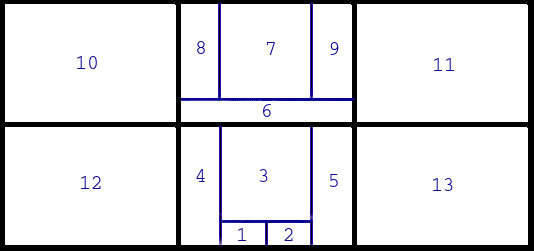
\includegraphics[scale=0.5]{imagenes/Regiones.jpg}
\caption{Campo de visión del robot con el número de cada región. Cada cuadro blanco demarcado con líneas negras representa la imagen captada desde una posición fija de la cámara. La región de pateo de la pelota se encuentra en las regiones 1 y 2 }
\label{divisionCam}
\end{figure}

\subsection{Comunicación Arbotix - Raspberry (ROS)}\label{comunicacion}

La Raspberry Pi procesa la información de la cámara y la Arbotix controla los actuadores. Para coordinar los movimientos del robot según la posición de la pelota se estableció una forma de comunicación entre ambas tarjetas. 

Se ha establecido la Arbotix como servidor de peticiones y a la Raspberry Pi como cliente. Dentro de la Raspberry Pi se ejecuta el proceso de decidir qué acción debe tomar el robot. Una vez determinada la acción se envía la petición a la Arbotix para que esta la ejecute. Este proceso es bidireccional y síncrono, es decir, la Raspberry envía la petición y se bloquea hasta que la Arbotix retorne la respuesta de su culminación.  

Para la implementación de la comunicación se ha usado ROS con su versión Hydro y se ha utilizado la interfaz de comunicación basada en servicios que no es más que un método de comunicación basado en el paradigma de resquest / reply con el concepto de maestro esclavo.

\subsection{Elecci\'on de la acci\'on}\label{eleccionAccionesFijas}

Una vez con la representaci\'on del mundo, los movimientos programados y la comunicaci\'on de las tarjetas, solo faltaría decidir que acci\'on tomar en cada situación. En primera instancia se ha decidido fijar una acción por cada región en la que se detecte la pelota. 

A continuación se especifica la acción a tomar en cada region: 
 \begin{itemize}
\item Girar a la Izquierda: Junny debe girar a la izquierda cuando la pelota se encuentre en alguna de las siguientes regiones: 4, 8, 10 y 12.

\item Girar a la Derecha: debe girar a la derecha cuando la pelota se ubique en alguna de las siguientes regiones: 5, 9, 11 y 13. 

\item Caminar hacia adelante: cuando la pelota se ubique en alguna de las siguientes regiones: 3, 6 y 7.

\item Patear con la pierna izquierda: cuando la pelota se encuentre en la región 1.

\item Patear con la pierna derecha: cuando la pelota se encuentre en la región 2.

En caso de no encontrar la pelota en ninguna de las regiones, el robot gira con los pies para cambiar su orientación física e iniciar nuevamente el movimiento de la cámara para hallar la pelota. Cuando se tiene la pelota en una posición cercana a los pies se realiza la acción de patear.
\end{itemize}